\section{Proof of Concept Implementation}\label{ch:implementation}
% +Implementation:
% *System:
% 	-Raspbian OS: distro de debian para Raspberry Pi, que se describirá en los tests
% 	-LEDE: ash terminal (shell command interpreter), POSIX, typical hardware, libraries with no hardware aceleration vs smart card MULTOS,
%
% *Delegation
%  -REST as current delegation protocol: curl script bash
%  -BIOSC as current APDU transmission protocol: no security -> no overload.
% *Smart Card
%  
%  -IoT Smart Card software design and implementation notes.
%  -Sequence diagrams. TODO


This section presents the first PoC implementation, introducing the IoT system used in the tests, the delegation protocols, one for the computation offloading of the IoT device on the P2ABCE server, and another one for the transmission of APDU Commands, and finally, the IoT smart card implementation.

The PoC is developed under a Linux based system aimed for IoT environments, a fork of OpenWrt, called LEDE (Linux Embedded Development Environment), that will serve as a starting point for future implementations in more constrained devices. 
The delegation server will run on Raspbian OS, in a Raspberry Pi 3, with a suitable Java Runtime for P2ABCE to run.


%%%Regarding the definition of the P2ABCE API, it is a work in progress, and in the meantime,         we           will work with the REST API currently available in the P2ABCE project to perform the delegation. Regarding the \textit{IoT Smart Card}, the P2ABCE project defines the APDU instructions with the corresponding format of the APDU Commands and Responses. In the next section we will explain the PoC for IoT based on these P2ABCE specifications.


%\subsection{PoC Delegation}

After the device receives a P2ABCE message from a third party actor, the delegation process begins. It consists on two steps, first the IoT device calls the P2ABCE server to offload the parsing of the XML data, and then the P2ABCE server, sending APDU Commands, delegates on the IoT smart card the cryptographic calculations, if needed.


\subsection{PoC Delegation to P2ABCE Server}


Currently the P2ABCE project offers multiple REST web services to run different roles in the P2ABCE system: User Service, Issuer Service, Verification Service, etc. These services make use of helper libraries that can be used to implement other services, with more suitable protocols for each specific deployment.

After an analysis of the project's code, the smart card logic was found in  the \texttt{Smartcard} interface and its implementations, \texttt{HardwareSmartcard} and \texttt{SoftwareSmartcard} classes. The first one uses the \texttt{javax.smartcardio} abstract classes to communicate with the physical smart cards. The Oracle JRE implements these package for the majority of smart card manufacturers. For our PoC, \texttt{javax.smartcardio} package was implemented, as \texttt{IoTsmartcardio}, so it transmits the APDU Commands and Responses with a simple custom protocol, making the use of a physical or IoT smart cards totally transparent to the \texttt{HardwareSmartcard} class, enhancing maintainability, and following the \textit{expert pattern} from the known GRASP guidelines.

In this PoC, the P2ABCE's User Service was modified to add a new method receiving the IoT device's  IP address and a port where the IoT Smart Card will be listening for the APDU Commands, the information needed for the custom protocol to transmit APDUs. 
The remaining REST methods of the services are left untouched.


\subsection{APDU Dialogue Transmission}

The transmission of APDU messages between the delegation server and the IoT device is done through a custom simple protocol, referred as BIOSC (Basic Input Output Smart Card).

It consists on one first byte for the instruction, that can mean either an APDU Commnad or a finishing instruction to close the connection. 
In the first case, the header continuous with two more bytes for the length of the payload bytes to read, which are the APDU Command bytes.
To send an APDU Response in BIOSC, the IoT device sends back to the server two bytes for the length and then the raw APDU Response bytes. The messages are sent over TCP for a reliable transmission.

The protocol lacks any security (authentication or authorization) that a real system should implement. It is vital to authenticate the delegation service, to authorize it to perform APDU Commands, and the same goes for the IoT device, to prevent impersonation attacks. But using BIOSC for the transmission of the APDU messages in the PoC, with only 3 bytes of overhead, will help in the  benchmarks to measure the performance of the system, independently of the connection to the delegation service.


\subsection{IoT Smart Card Implementation}

This section showcases the code architecture and sequence diagrams of the IoT Smart Card PoC.

%\hfil
%
%\textsc{Code structure}

Figure~\ref{fig:IoTCScomponents-color} shows how the project is divided in three different sections, with the objective of enhancing maintainability, improving future changes, ports and error fixes.


\begin{figure}[bth]
	\centering
	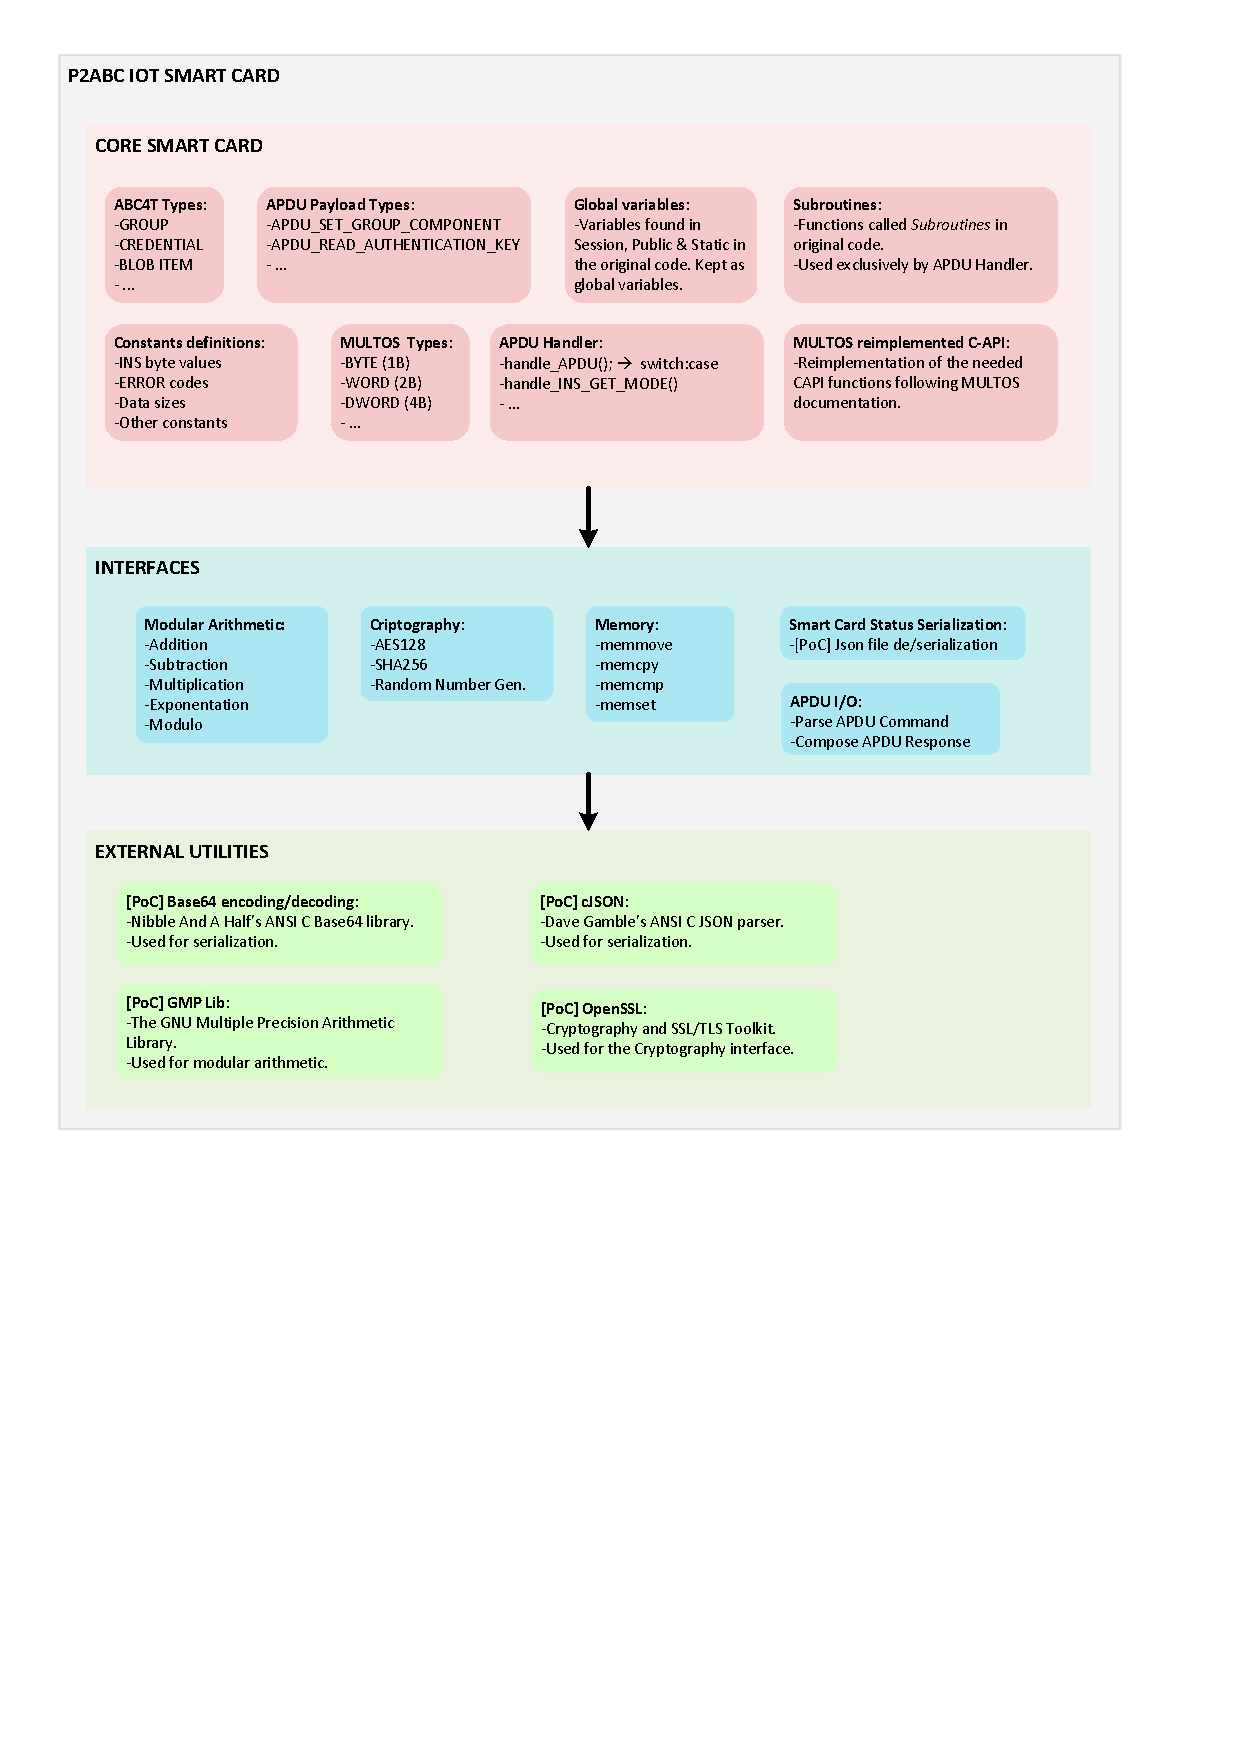
\includegraphics[width=\linewidth]{gfx/IoTCScomponents-color}
	\caption{IoT Smart Card Code Structure.}
	\label{fig:IoTCScomponents-color}
\end{figure}


\textbf{Core smart card:} The smart card logic lies here, with the concepts of APDU Commands and Responses, the instructions that are defined for P2ABCE smart cards, and how to process them and perform the cryptographic calculations.

It is mainly based on ABC4Trust Card Lite's code, a MULTOS physical smart card implementation of P2ABCE smart cards, but also on the \texttt{SoftwareSmartcard} Java implementation for a high level reference. MULTOS acts as an operative system for smart card applications. It provides a custom API for memory management, arithmetic functions, etc. It also uses an architecture different from traditional computers. This implied an almost integral reimplementation of the original code.

In some cases, to  avoid some MULTOS API limitations, like in \cite{vullers2013efficient} where they noted that MULTOS' \texttt{ModularExponentiation} did not accept exponents larger than the modulus size, an equivalent function with \textit{expanded functionality} was implemented. 

Another notable difference is that MULTOS compiler does not apply data structure alignment. This affects the inherited ABC4Trust's code because of the massive use of \texttt{memcpy} to copy multiple adjacent variables with one function call, usually when reading or writing APDUs. 
A temporal solution is to use \texttt{struct \_\_attribute\_\_((\_\_packed\_\_))} to ask the GCC compiler not to use padding in the structs, but this is not standard functionality, neither a good practice. A deeper refactorization of the code would be needed where the obscured copies of variables must be made explicit, letting the compiler manage the memory layout on its own.

\hfil

\textbf{Interfaces:} To reimplement some of the MULTOS functions, a facade isolates the implementation of the core smart card from auxiliary function implementations, that could vary depending on the hardware or the system used by the IoT device.
With this facade, for example, it could be possible to change the implementation of cryptographic functions to use hardware acceleration (e.g. Atmel's chips for SHA and AES), or new software implementations optimised for the target platform.

The interfaces defined can be organized in 5 groups (see Fig.~\ref{fig:IoTCScomponents-color}), depending on their purpose: Modular Arithmetic, Cryptography, Memory Management, Serialization and APDU Parsing.

\hfil

\textbf{External utilities:} To implement some \textit{interfaces}, the current PoC uses two ANSI C libraries, for base64 and JSON, and two shared libraries available as packages in LEDE: GMPLib and OpenSSL. These libraries use dynamic memory and offer more functionality than what is actually needed, and although they are useful tools for the early development versions of the PoC, future versions should replace them for more lightweight solutions.

\hfil

The \textit{interfaces} and \textit{external utilities} sections  allow that the project is easily ported to specific targets without modifying the smart card logic.


\hfil

%\textsc{Execution workflow}

The sequence diagram from Figure~\ref{fig:sequenceBIOSC} shows the execution of the PoC IoT smart card.



\begin{figure*}[bth]
	\centering
	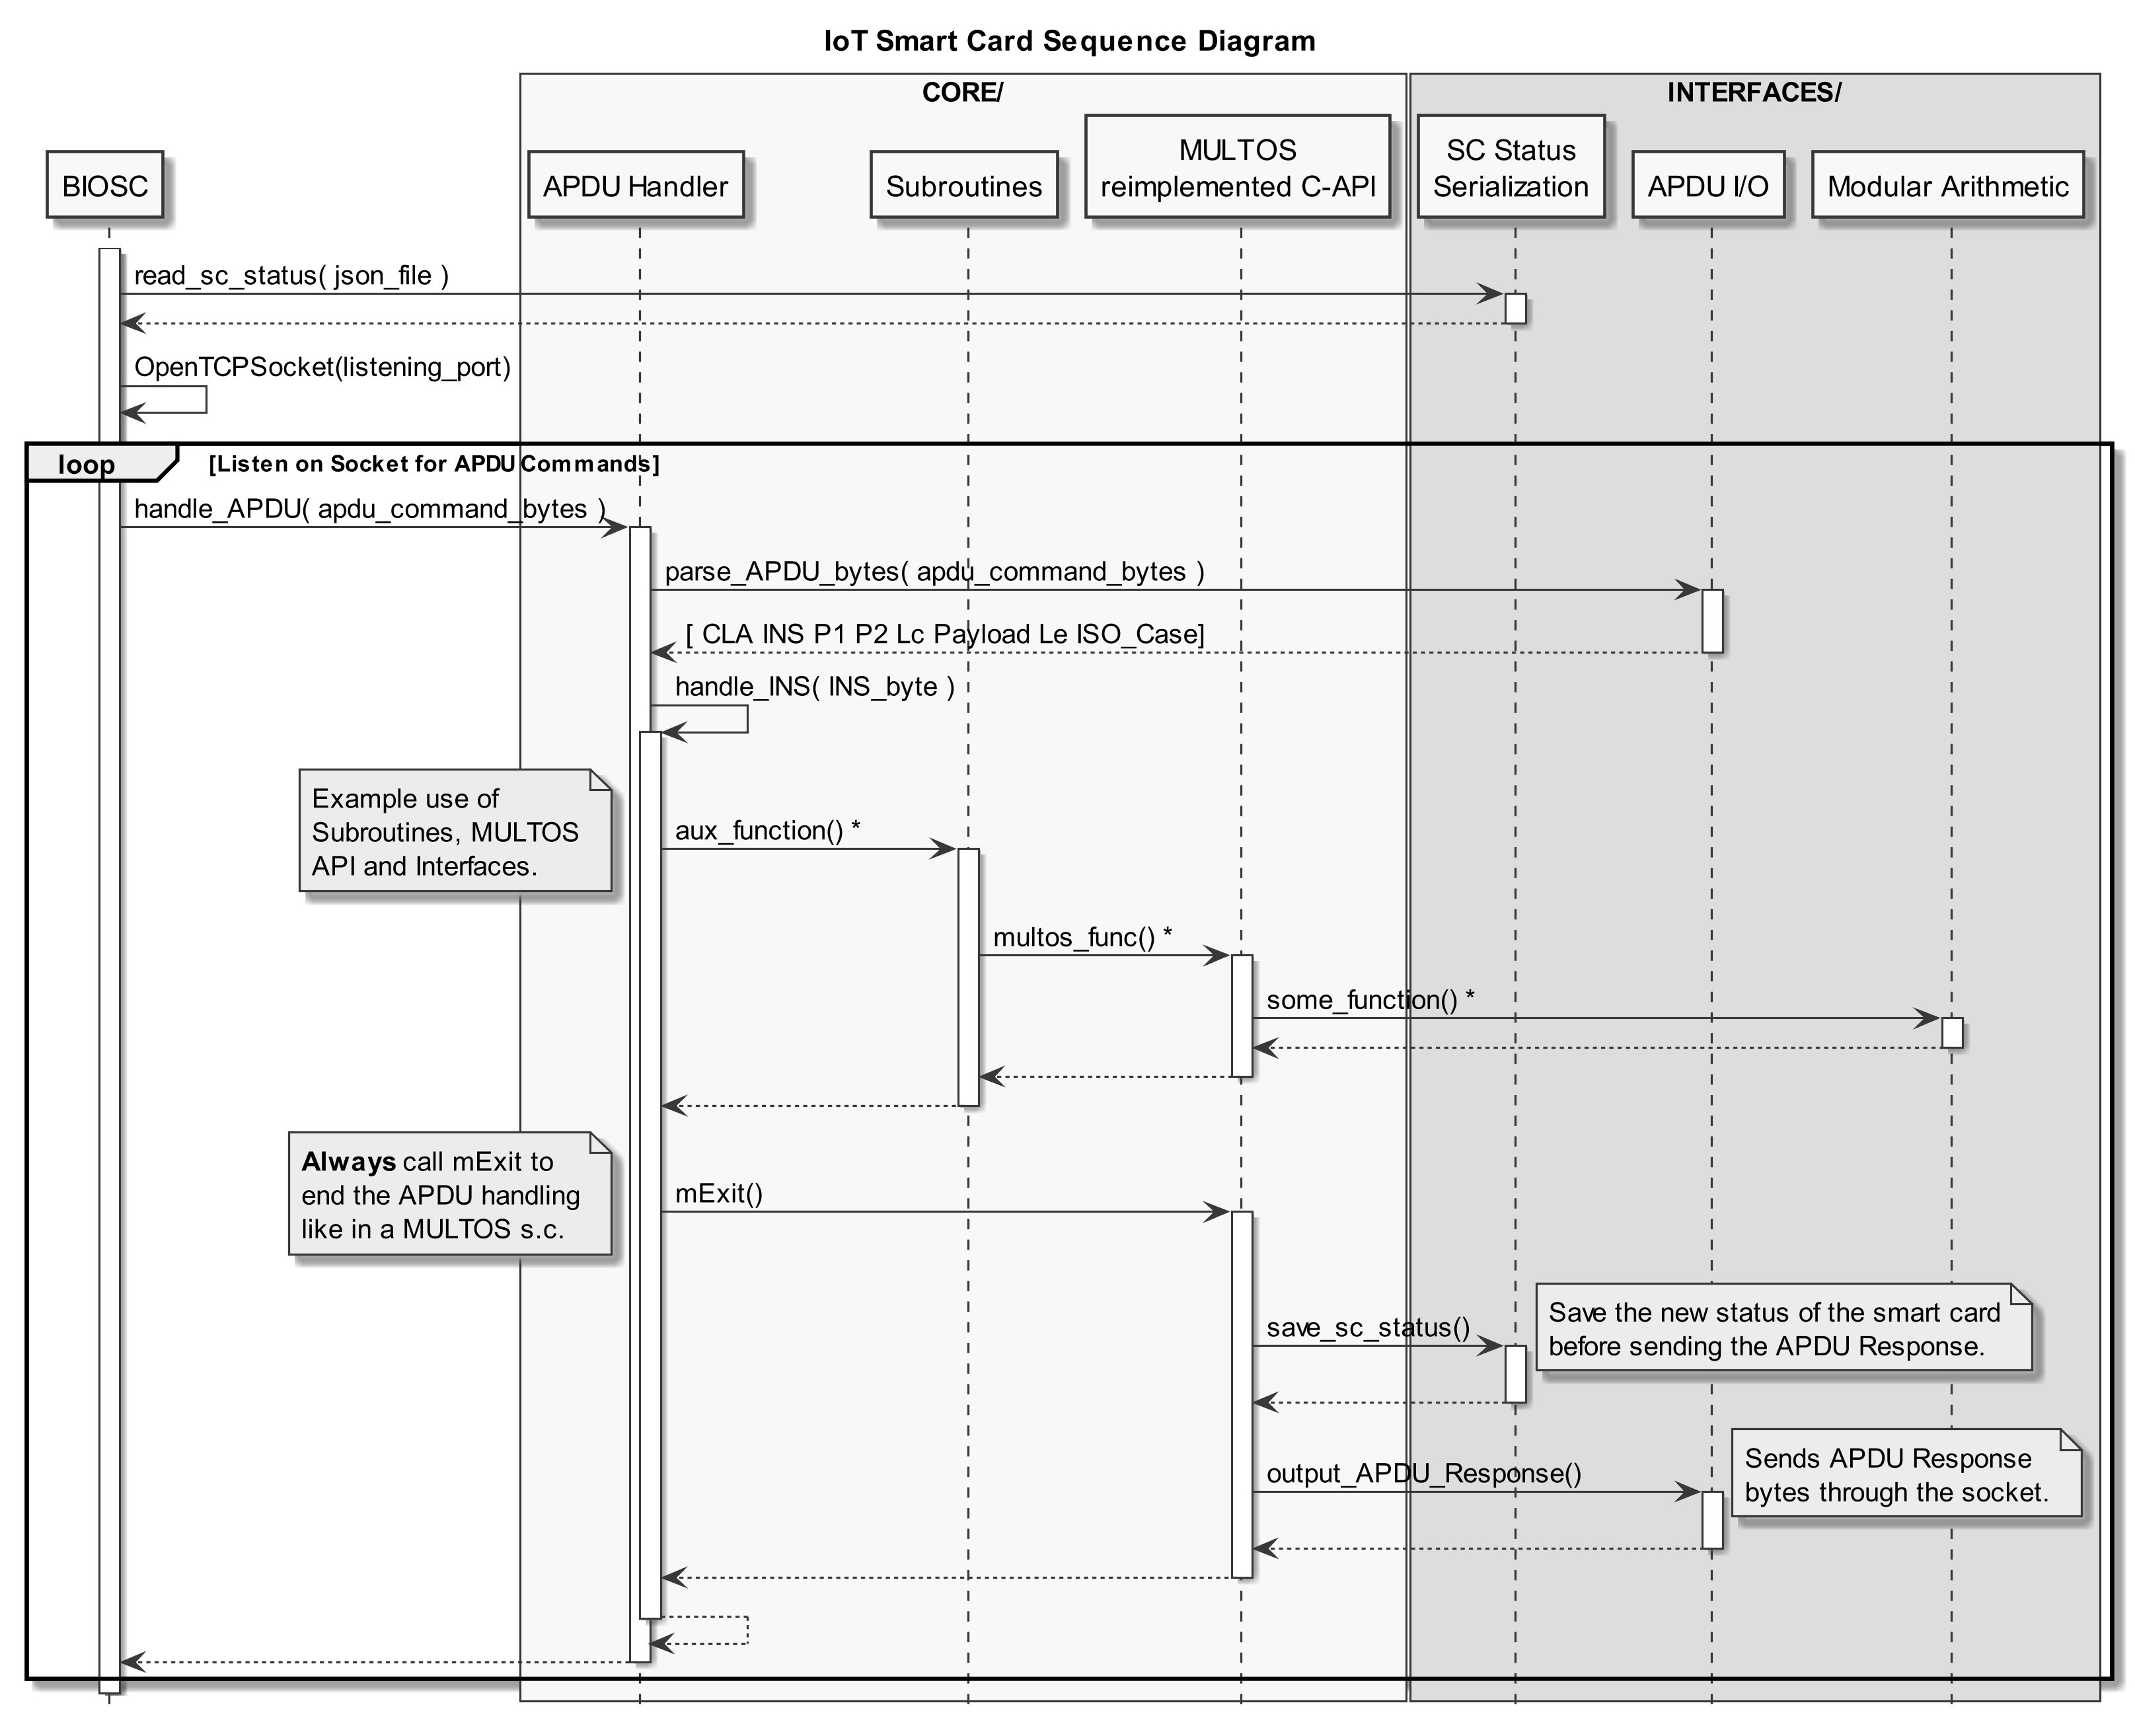
\includegraphics[width=0.8\textwidth]{gfx/UML/sequenceBIOSC}
	\caption{IoT Smart Card Sequence Diagram.}
	\label{fig:sequenceBIOSC}
\end{figure*}



The execution starts with the \texttt{main} function in \texttt{BIOSC.c}, first it deserializes the current smart card status from a Json file (which helps with debugging the IoT smart card), next, it listens on a loop for APDU Commands from the delegation server.

Every time an APDU Command arrives, it calls the function \texttt{handle\_APDU()} with the raw APDU bytes. The Handler calls the APDU I/O interface to parse the bytes, storing in different variables the APDU structure. Using a \texttt{switch-case} expression on the \texttt{INS} byte, the Handler calls a fitting \textit{Instruction handler} function.

Inside this function, it may call multiple functions from the Subroutines, that may call MULTOS C-API functions, which, in turn, may use an interface to perform its functionality, depending on the specific instruction being handled.

Finally, every instruction handler must end. Right before the \texttt{return;} expression, they must call \texttt{mExit}. This reimplemented MULTOS function will save the current status of the smart card and send the formed APDU Response to the delegation server.

After returning from the APDU handler, the program listens again from the socket, until a BIOSC finishing instruction arrives.


